% --- TITELSEITE DESIGN ---
\thispagestyle{empty} % Keine Seitenzahlen auf dem Titel

% Lade die automatischen Daten (falls Skript nicht lief, Dummy Werte)
\IfFileExists{generated/title_data.tex}{
    % Automatisch generierte Daten (1. + 2. Mannschaft)

\newcommand{\TitelSpieltage}{22. Spieltag / Kreisliga 1}
\newcommand{\TitelDatume}{Sonntag 12.04.2026 | 14:00 Uhr}
\newcommand{\TitelPartiee}{SV Obertraubling - SV Burgweinting Rgbg.}

\newcommand{\TitelSpieltageII}{22. Spieltag / A-Klasse 2}
\newcommand{\TitelDatumeII}{Sonntag 12.04.2026 | 16:00 Uhr}
\newcommand{\TitelPartieeII}{SV Obertraubling II - VfR Regensburg II}

% Ausgabe Nummer (global)
\newcommand{\TitelAusgabeNr}{Ausgabe Nr. 10, Saison 25/26}

}{
    \newcommand{\TitelSpieltag}{Spieltag ??}
    \newcommand{\TitelDatum}{Datum ??}
    \newcommand{\TitelPartie}{Heim - Gast}
    \newcommand{\TitelAusgabeNr}{Ausgabe Nr. 0}
}

\begin{tikzpicture}[remember picture, overlay]
    % Koordinatenursprung oben links
    \node[anchor=north west, inner sep=0] at (current page.north west) {};

    % --- 1. HEADER BEREICH ---
    
    % Logo Rechts Oben
    \node[anchor=north east] at ([xshift=-1.5cm, yshift=-1.5cm]current page.north east) {
        \includegraphics[width=3.5cm]{bilder/logos/no_border.png} % Pfad anpassen!
    };

    % Schriftzug "O-TON" (Rot)
    \node[anchor=north west] at ([xshift=2cm, yshift=-2.5cm]current page.north west) {
        \fontsize{70}{80}\selectfont \bfseries \color{VereinsRot} O-TON
    };

    % Slogan Text (Blau)
    \node[anchor=north west, align=left] at ([xshift=2cm, yshift=-5.5cm]current page.north west) {
        \color{VereinsBlau} \large {Obertraubling - Rauben \& Brandschatzen} \\
        \\[0.5em]
        \color{VereinsBlau} \large {\TitelAusgabeNr}
    };

    % --- 2. BLAUER FOOTER (DIE WELLE) ---
    
    % Wir malen den blauen Bereich unten.
    % Wir starten unten links, gehen nach rechts, hoch und machen eine Kurve.
    \fill[VereinsBlau] 
        (current page.south west) rectangle ([yshift=11cm]current page.south east);
        
    % Wir schneiden oben eine Kurve raus (Trick: Wir malen Weiß darüber)
    % Das hier erzeugt die Kurve zwischen Bild und blauem Bereich
%    \fill[white] 
%        ([yshift=10cm]current page.south west) 
%        .. controls ([xshift=5cm, yshift=-2cm]current page.center) and ([xshift=10cm, yshift=2cm]current page.center) .. 
%        ([yshift=14cm]current page.south east)
%        -- (current page.north east) -- (current page.north west) -- cycle;


    % --- 3. DAS FOTO (BESCHNITTEN) ---
    
    % Wir definieren einen Clipping-Pfad (Die Form des Bildes)
    \begin{scope}
        % Die Form: Ein Oval/Linse, das oben in das Weiße reinragt
        % Dies ist etwas Fummelarbeit mit den Koordinaten, bis es passt
%        \path[clip] 
%            ([xshift=1cm, yshift=10.5cm]current page.south west) 
%            to[out=15, in=165] ([xshift=-1cm, yshift=14.5cm]current page.south east) % Obere Kurve
%            to[out=-80, in=80] ([xshift=-1cm, yshift=8cm]current page.south east)   % Rechts runter
%            to[out=195, in=-15] ([xshift=1cm, yshift=4cm]current page.south west)    % Untere Kurve (Die Welle)
%            -- cycle;
%            
        % Das Bild selbst
        \node at (current page.center) [yshift=0cm] {
            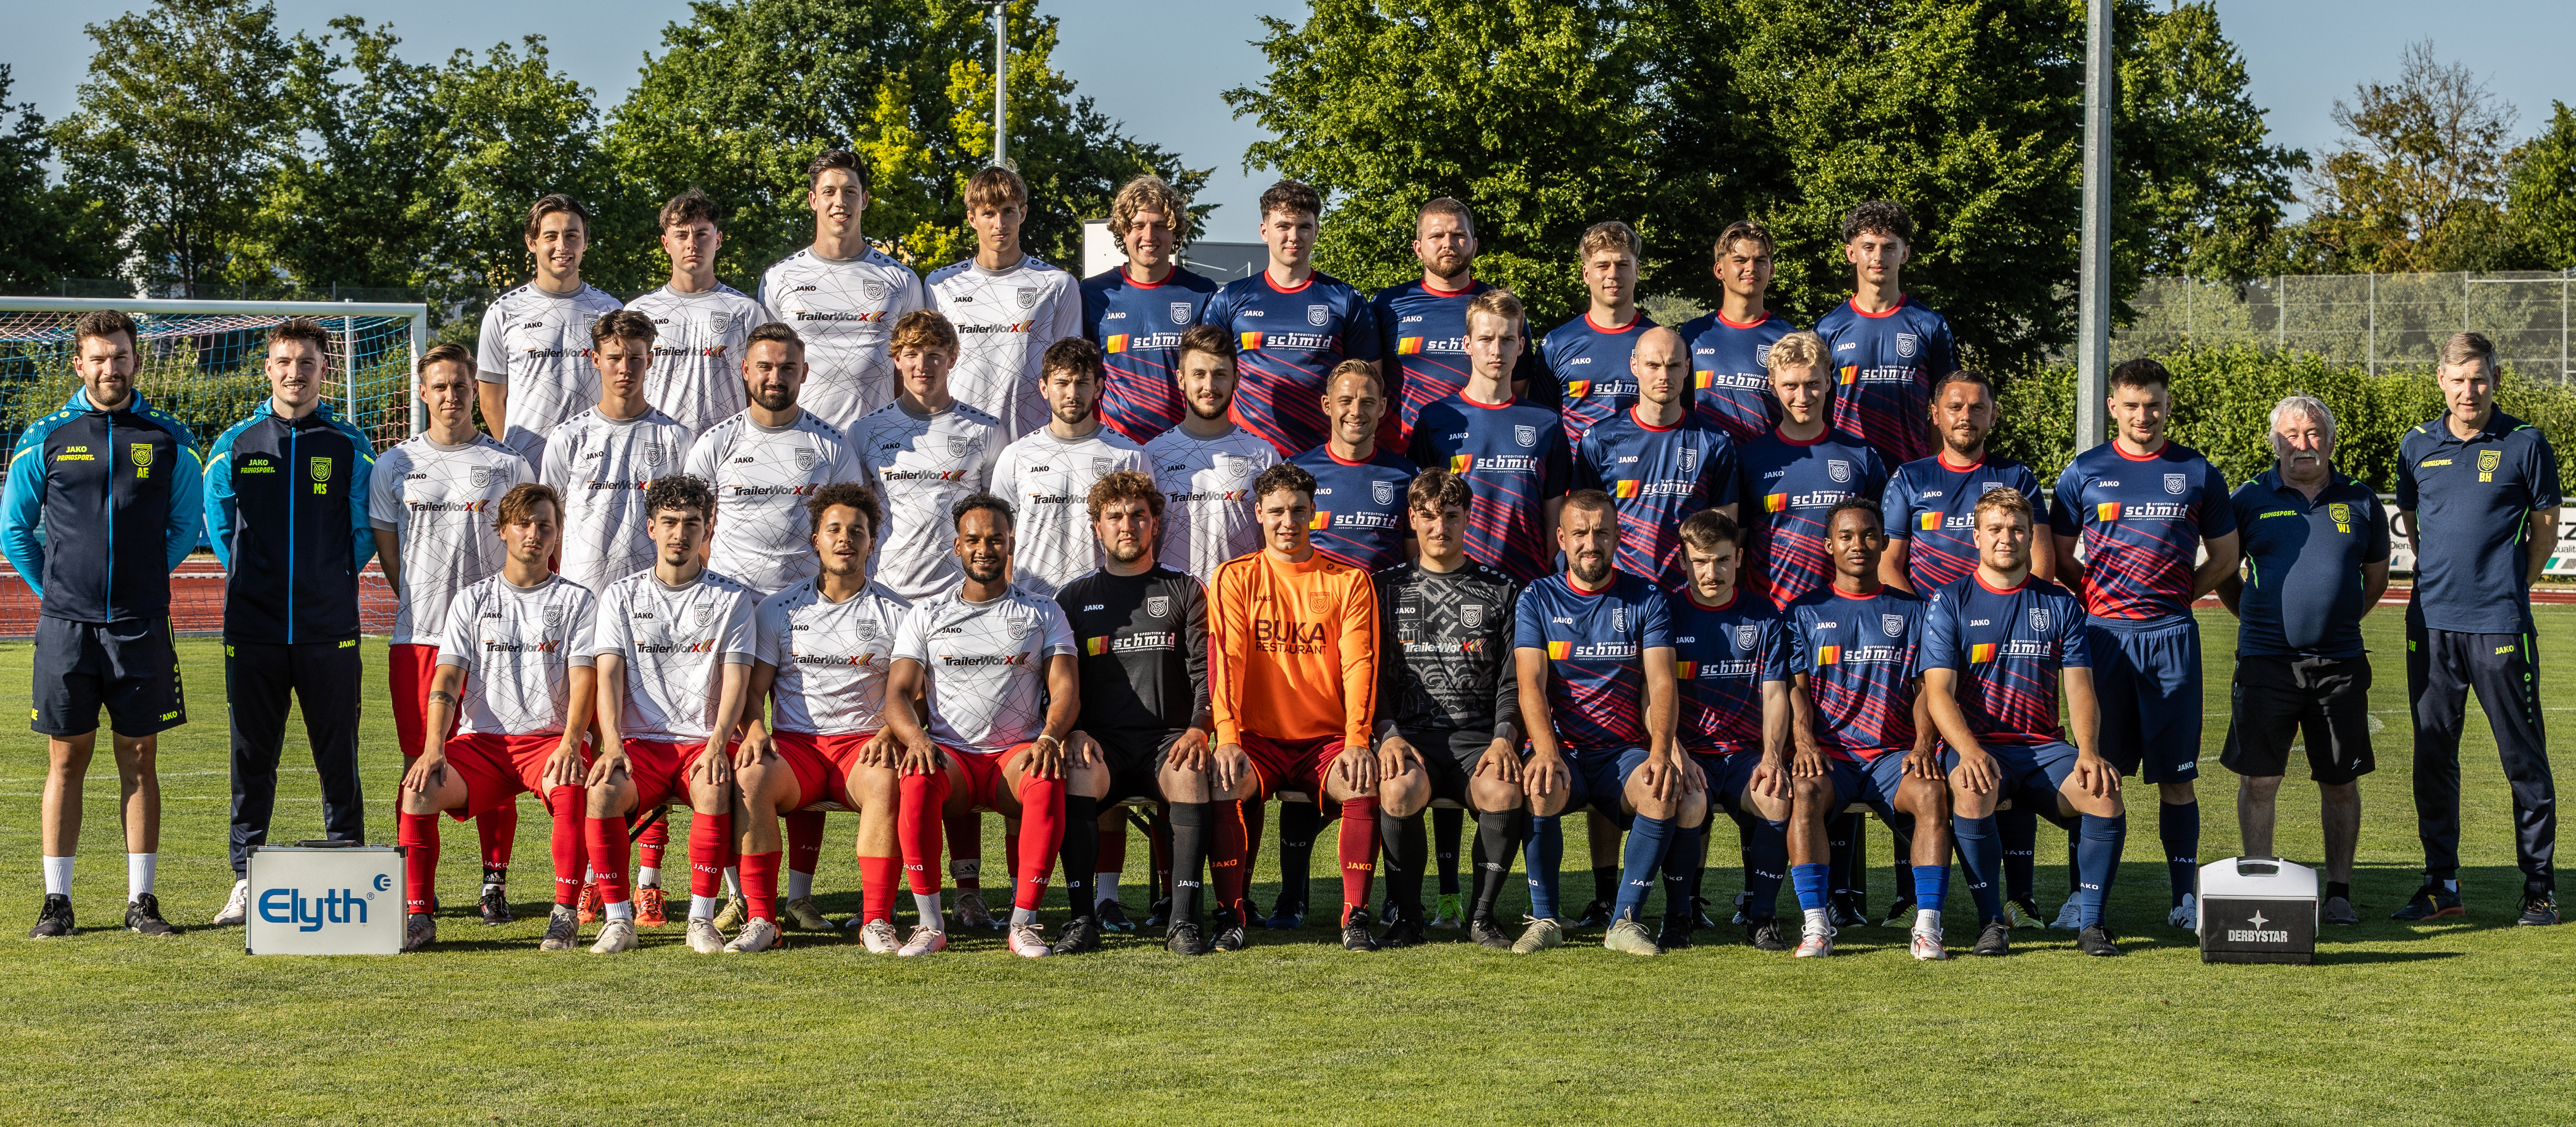
\includegraphics[width=\paperwidth]{bilder/mannschaft.png} % Dein Foto
        };
        
        % Weiße Konturlinien (die "Swooshes" unter dem Bild)
%        \draw[white, line width=3pt] 
%             ([xshift=0cm, yshift=4cm]current page.south west) 
%             to[out=15, in=195] ([xshift=0cm, yshift=8cm]current page.south east);
    \end{scope}

    % --- 4. TEXT IM FOOTER (WEISS) ---
    
    % Block 1: Kreisliga
    \node[anchor=west, align=left, text=white] at ([xshift=2cm, yshift=6cm]current page.south west) {
    \color{white}
        \fontsize{20}{24}\selectfont \textbf{\TitelSpieltage} \\[0.5em]
        \color{white}
        \Large \TitelDatume \\[0.3em]\color{white}
        \Large \textbf{\TitelPartiee}
    };

    % Block 2: A-Klasse (Statisch oder zweite Variable)
    \node[anchor=west, align=left] at ([xshift=2cm, yshift=3cm]current page.south west) {
  \color{white}
  \fontsize{20}{24}\selectfont \textbf{\TitelSpieltageII} \\[0.5em]
  \color{white}
  \Large \TitelDatumeII \\[0.3em]
  \color{white}
  \Large \textbf{\TitelPartieeII}
};

\end{tikzpicture}
\newpage